\section{Evalution}
\label{exp}
We evaluate the implementations on two platforms. The first is the  NVIDIA Tesla K40m, which facilitates 2880 FP32 cores with a 64KB L1 cache and
shared memory. The host machine has a 2.40GHz Intel Xeon E5-2620 CPU with 128GB memory and Linux kernel v4.19.85. The second platform is the NVIDIA RTX 2080 Ti, which facilitates 4350 FP32 cores and 4350 INT32 cores with a 96KB L1 cache and shared memory. The host machine has a 2.30GHz Intel Xeon E5-2697
CPU with 252GB memory and Linux kernel v4.15.0. Both platforms are shipped with the CUDA Toolkit v10.1. We use the following state-of-the-art convolution libraries for comparison on both platforms:
\begin{itemize}
  \item cuDNN, version 7.6. cuDNN is a state-of-art convolution implementation that supports 2D and 3D convolutions on GPU.
      Moreover, cuDNN can execute GEMM-, FFT- and Winograd-based convolutions.
  \item GEMM-im2col (im2col) and GEMM-im2row (im2row). Both are GEMM-based convolutions and support 2D and 3D convolutions.
      We extract the implementations of the im2col and im2row from Caffe \cite{jia2014caffe} and MatConvNet \cite{vedaldi15matconvnet}, respectively.
  \item ArrayFire \cite{Yalamanchili2015}, version 3.6.4. ArrayFire is a popular image and signal processing library. This library implements 2D
      convolutions on GPU and can be easily invoked through API. The semantics of the 3D convolution in ArrayFire is not compatible with the 3D
      convolutions in CNNs. Therefore, we use ArrayFire for 2D convolution only. ArrayFire uses Just In Time compiling for standard
      arithmetic operations; thus, the first run of an ArrayFire application takes longer than the second run.
      In the experiment, we run ArrayFire twice in each test and record the second runtime.
  \item NVIDIA Performance Primitives (NPP), version 10.1. NPP is an image and signal processing library. We use NPP for 2D convolutions only because we cannot find functions for performing 3D convolution.

\end{itemize}

After years of updating, cuDNN has integrated seven widely used convolution algorithms. Therefore, cuDNN provides an option that uses
heuristics to find the most suitable algorithm for a convolution. We set the option to $PREFER\_FASTEST$ (the exact option can be found at
\cite{CUDAtoolkit}); that is, we prefer to use the fastest algorithm regardless of the memory capacity. However, the algorithm
selected by the heuristic is not always the fastest. Therefore, we use two types of runtime for cuDNN. One is the real fastest runtime
among the seven algorithms and the other is the heuristically fastest runtime. For 2D convolutions, we use the real fastest runtime because two types of runtime are the same.

%Our implementations of convolution use only a small part of shared memory and mainly relay on GPU L1 cache. Therefore we employ $cudaDeviceSetCacheConfig$ function to set GPU cache policy with arguments $cudaFuncCachePreferL1$ for our convolutions.
All experiments use a 32-bit float data type and an average runtime of 10 iterations. All data are 4D tensors $(N,C,H,$ and $W)$. For
now, we implement the 2D and 3D convolutions with one and three input channels for the filters with sizes $3 \times 3$ and $5 \times 5$, respectively, because small filters are commonly used in applications. The results for the 2D convolution and are presented first in the subsequent section, followed by that for the 3D convolution.

\subsection{2D Convolution}
\begin{figure*}
\begin{subfigure}{\columnwidth}
		\centering
		 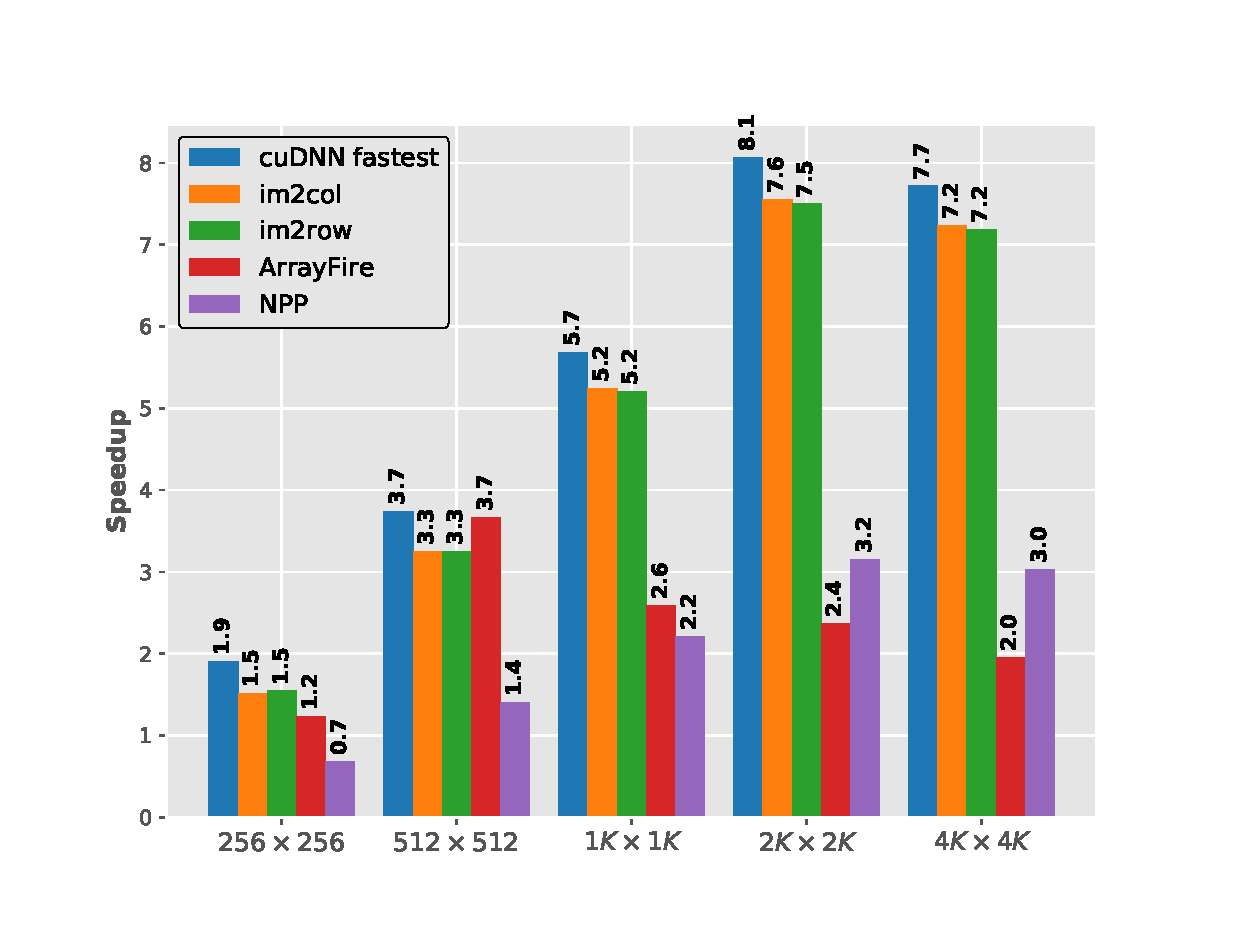
\includegraphics[width=\columnwidth,height=6cm]{./figure/2d_norm_f3.eps}
		 \caption{Speedups for the filter of size $3 \times 3$ on Tesla K40m.}
		 \label{fig:2druntimef3c1}
	\end{subfigure}
	\begin{subfigure}{\columnwidth}
		\centering
		 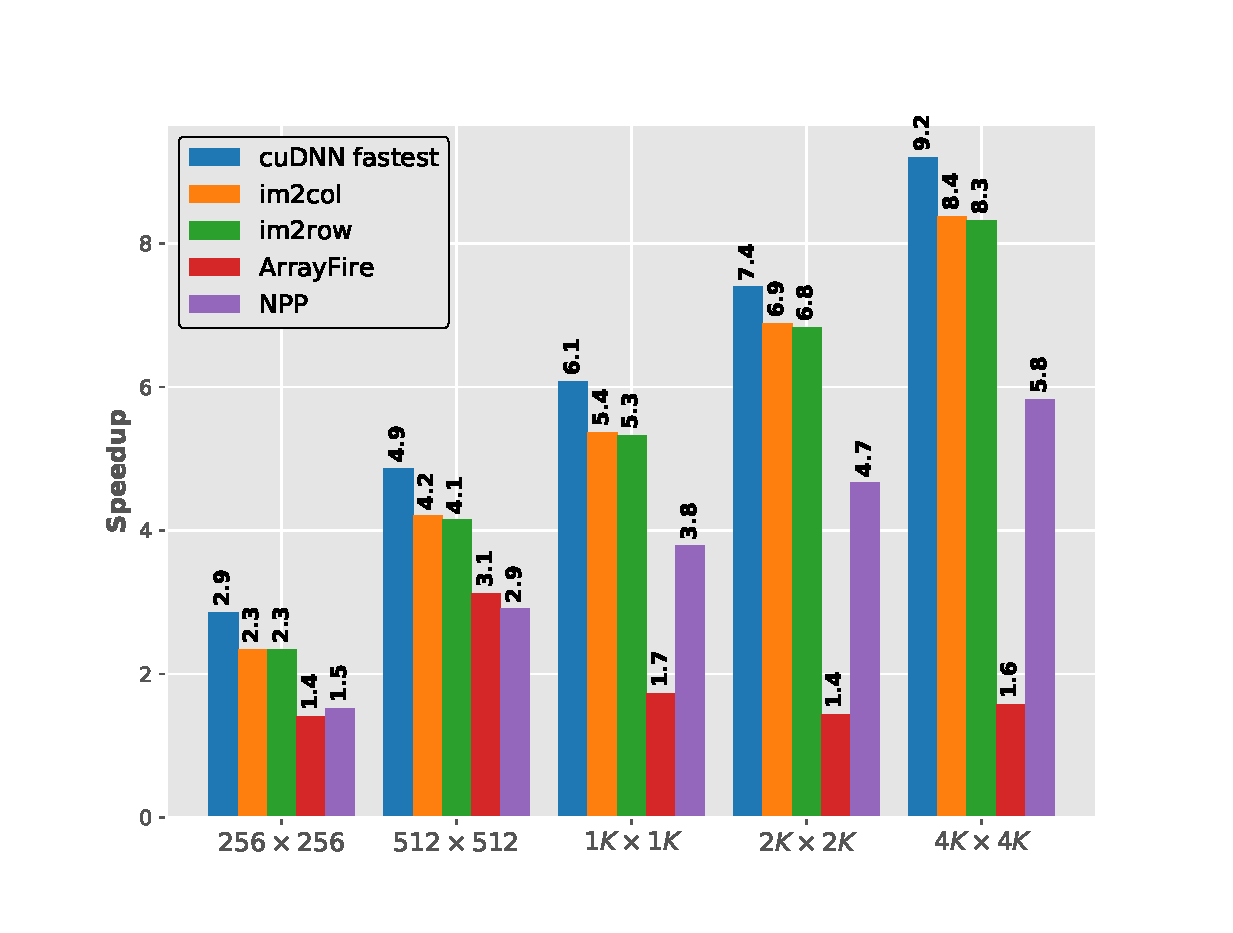
\includegraphics[width=\columnwidth,height=6cm]{./figure/2d_norm_f5.eps}
		 \caption{Speedups for the filter of size $5 \times 5$ on Tesla K40m.}
		 \label{fig:2druntimef5c1}
	\end{subfigure}
	
	\begin{subfigure}{\columnwidth}
		\centering
		 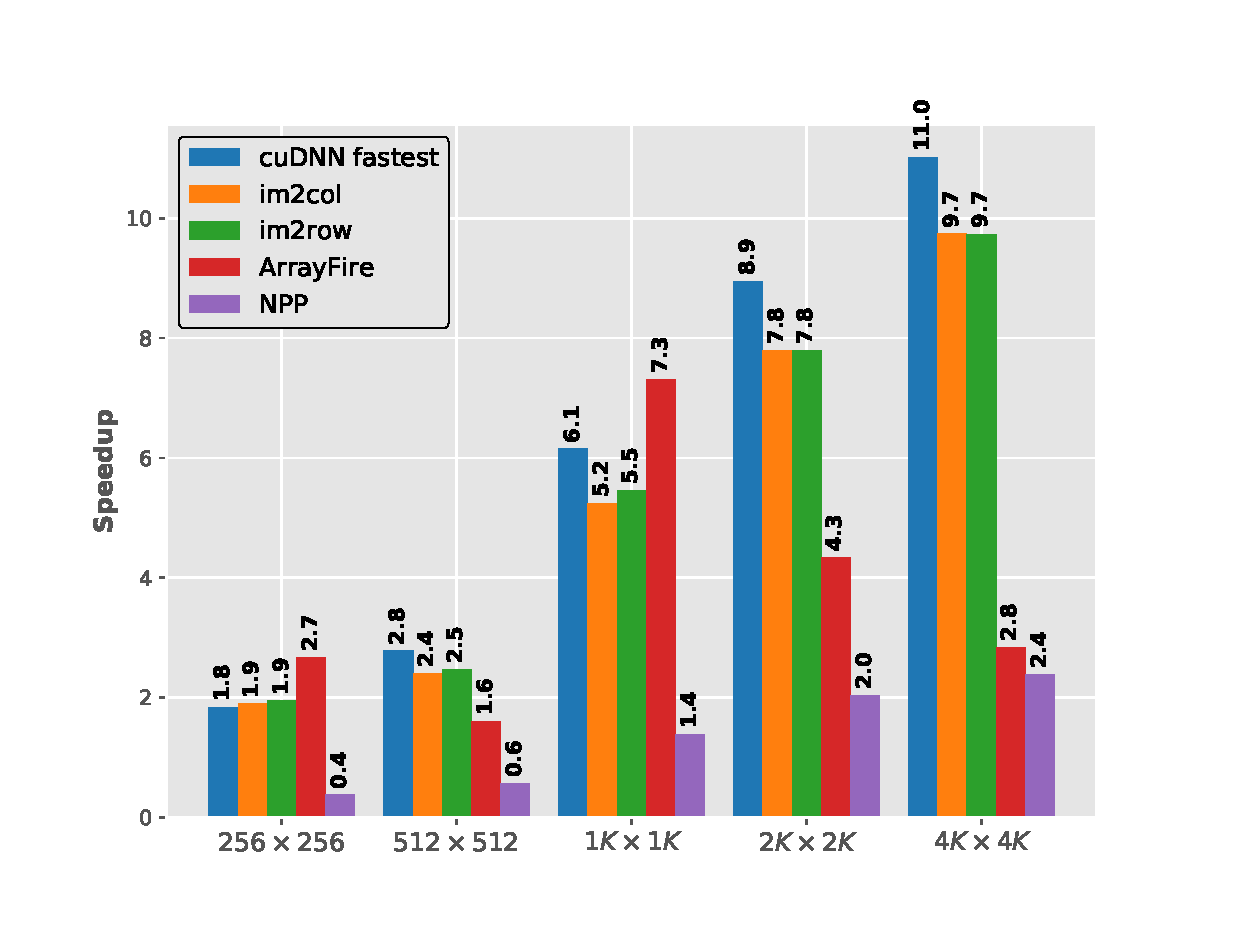
\includegraphics[width=\columnwidth,height=6cm]{./figure/2d_norm_f3_rtx2080.eps}
		 \caption{Speedups for the filter of size $3 \times 3$ on RTX 2080 Ti.}
		 \label{fig:2druntimef3c12080}
	\end{subfigure}
	\begin{subfigure}{\columnwidth}
		\centering
		 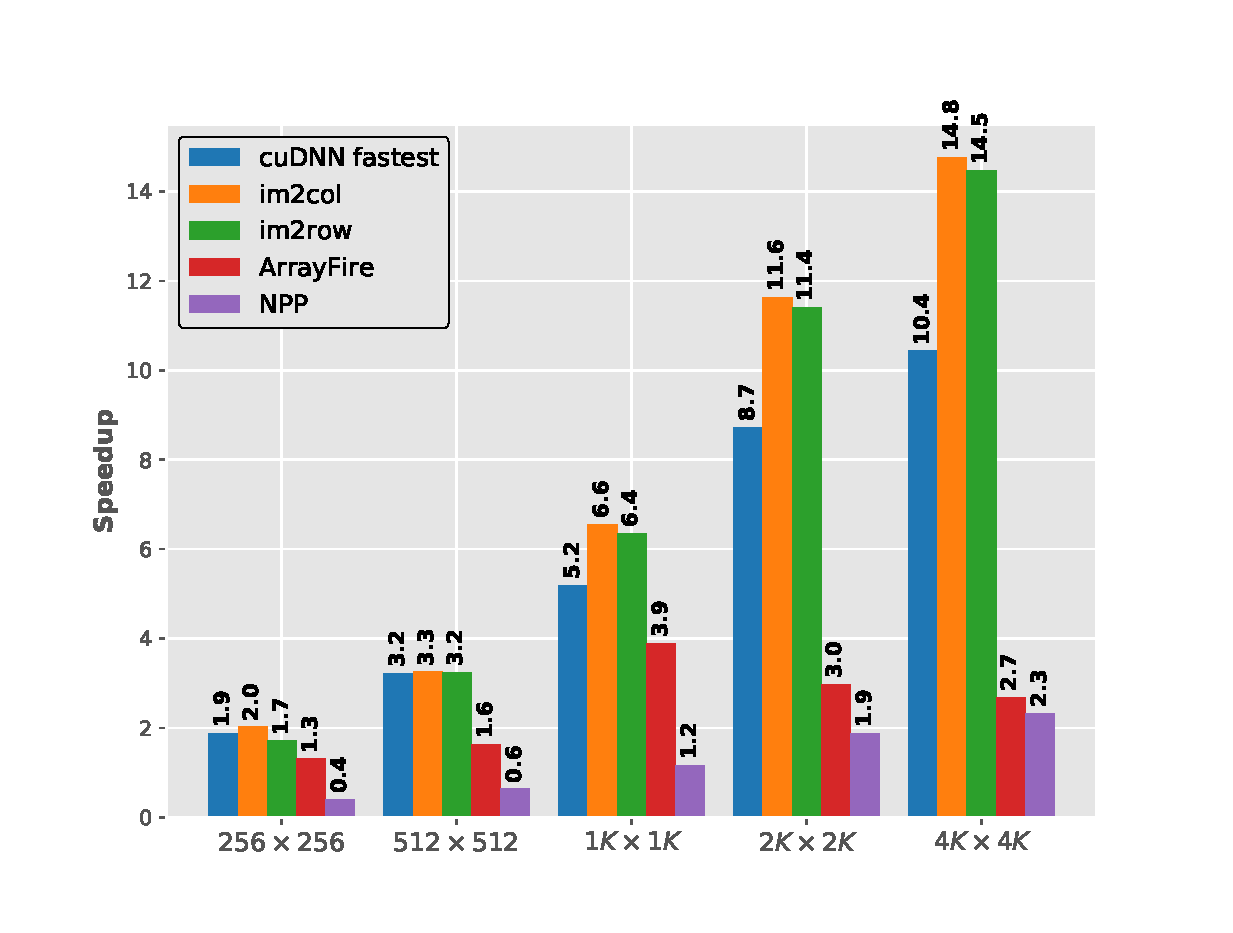
\includegraphics[width=\columnwidth,height=6cm]{./figure/2d_norm_f5_rtx2080.eps}
		 \caption{Speedups for the filter of size $5 \times 5$ on RTX 2080 Ti.}
		 \label{fig:2druntimef5c12080}
	\end{subfigure}
	
	\caption{Speedups of our implementation over the other five 2D convolution implementations on two platforms.}
   \label{fig:2druntime}
\end{figure*}

\begin{table*}[]
\caption{Summation of memory transactions on each type of memory, including global memory, texture memory and shared memory. Data is collected on Tesla K40m.}
\label{tab:2dmemtrans}
\begin{tabular}{c|ccccc|ccccc}
\hline
\multicolumn{1}{l|}{}                                  & \multicolumn{5}{c|}{Filter size $3 \times 3$}                                                & \multicolumn{5}{c}{Filter size $5 \times 5$}                                                \\ \hline
                                                       & $256 * 256$      & $512 * 512$      & $1K * 1K$        & $2K * 2K$        & $4K * 4K$        & $256 * 256$      & $512 * 512$      & $1K * 1K$        & $2K * 2K$        & $4K * 4K$        \\ \hline
cuDNN                                                  & 6.0E+05          & 2.4E+06          & 9.7E+06          & 3.9E+07          & 1.5E+08          & 1.4E+06          & 5.6E+06          & 2.2E+07          & 8.9E+07          & 3.6E+08          \\
 im2col & 1.1E+05          & 4.4E+05          & 4.4E+05          & 7.0E+06          & 2.8E+07          & 2.3E+05          & 9.3E+05          & 3.7E+06          & 1.5E+07          & 6.0E+07          \\
im2row & 1.1E+05          & 4.4E+05          & 4.4E+05          & 7.0E+06          & 2.8E+07          & 2.3E+05          & 9.3E+05          & 3.7E+06          & 1.5E+07          & 6.0E+07          \\
ArrayFire                                              & 4.9E+04          & 2.0E+05          & 7.9E+05          & 3.2E+06          & 1.3E+07          & 1.1E+05          & 4.2E+05          & 1.7E+06          & 6.8E+06          & 2.7E+07          \\
NPP                                                    & 6.0E+04          & 2.4E+05          & 9.6E+05          & 3.8E+06          & 1.5E+07          & 1.3E+05          & 5.2E+05          & 2.1E+06          & 8.3E+06          & 3.3E+07          \\
Ours                                                   & \textbf{7.5E+03} & \textbf{2.7E+04} & \textbf{1.1E+05} & \textbf{4.2E+05} & \textbf{1.6E+06} & \textbf{1.0E+04} & \textbf{3.3E+04} & \textbf{1.3E+05} & \textbf{4.9E+05} & \textbf{1.9E+06} \\ \hline
\end{tabular}
\end{table*}

This section presents the performance of the 2D convolution obtained from six implementations, including cuDNN, im2col, im2row, ArrayFire,
NPP and the proposed method. We evaluate the six implementations with an image size ($I_H \times I_W$) ranging from $256 \times 256$ to $4K \times 4K$, $I_N=F_N=1$ and $I_C=F_C=1$. We first present the speedups of our implementation over the other five approaches in Figure \ref{fig:2druntime}. Then we show the effectiveness of our implementation on reducing the number of memory transactions in Table \ref{tab:2dmemtrans}.

Figure \ref{fig:2druntime} indicates that cuDNN, im2col and im2row are not suitable for 2D convolutions in contrast to ArrayFire, NPP and the proposed implementation. Our implementation exhibits superior performance over cuDNN, im2col and im2row on the
two platforms, with an average of 5.9$\times$, 5.9$\times$ and 5.8$\times$ speedups, respectively.

Figure \ref{fig:2druntimef3c1} and \ref{fig:2druntimef5c1} present the speedups on Tesla K40m in which the proposed method achieves the best results in nine cases out of ten. Our implementation is  slower than NPP when performing a $3 \times 3$ convolution on a $256 \times 256$ image. The average speedups of our implementation over ArrayFire and NPP on Tesla K40m are 2.1$\times$ and 2.9$\times$, respectively.
Figure \ref{fig:2druntimef3c12080} and \ref{fig:2druntimef5c12080} show the speedups on RTX 2080 Ti, in which the proposed implementation achieves the best
results in six cases out of ten. NPP achieves the best results on small image sizes, whereas our implementation demonstrates the
best results on large image sizes. The average speedups of our implementation over ArrayFire and NPP on RTX 2080 Ti are 3.1$\times$ and 1.3$\times$, respectively.

Our implementation of the 2D convolution is derived from direct convolution. We use column (Algorithm \ref{algo:basic}, Algorithm \ref{algo:basic2}) and row reuse (Algorithm \ref{algo:rowreuse}) on direct convolution. Hence, the performance gains are mainly attributed to the reduction on the number of memory transactions. We use \emph{nvprof} to collect the number of memory transactions for the different types of memories. The GPU global memory is used to store the input data in im2col, im2row, ArrayFire and our implementation. NPP and cuDNN utilize texture memory to store input data, whereas shared memory is normally used to store filter data. Therefore, we sum up the number of read transactions of the three memory types and report the results in Table
\ref{tab:2dmemtrans}. To save space, we only show the result of the memory transactions collected on Tesla K40m because the result on RTX 2080 Ti exhibits a similar trend.

The results in Table \ref{tab:2dmemtrans} verify that our optimization algorithms significantly reduce the number of memory transactions.
Compared with ArrayFire and NPP, which are well optimized for 2D convolutions, our implementation can respectively reduce the memory transactions by a factor of 10.2 and 12.3 on average.


% Please add the following required packages to your document preamble:
% \usepackage{multirow}


%\begin{table*}[]
%\caption{2d speedup}
%\label{tab:2dspeedup}
%\begin{tabular}{c|ccccc|ccccc}
%\hline
%\multicolumn{1}{c}{}&\multicolumn{5}{c}{$F_H*F_W= 3*3$} &\multicolumn{5}{c}{$F_H*F_W= 5*5$}\\
%\hline
%           & 256*256&512*512&1K*1K&2K*2K&4K*4K&256*256&512*512&1K*1K&2K*2K&4K*4K\\
%\hline
%cuDNN      & 1.91 & 3.74 & 5.69 & 8.07 & 7.72     & 2.86 & 4.86 & 6.08 & 7.40 & 9.20  \\
%im2col     & 1.52 & 3.25 & 5.25 & 7.56 & 7.24     & 2.34 & 4.20 & 5.37 & 6.88 & 8.38  \\
%im2row     & 1.55 & 3.25 & 5.20 & 7.50 & 7.19     & 2.34 & 4.15 & 5.32 & 6.83 & 8.32  \\
%ArrayFire  & 1.23 & 3.67 & 2.59 & 2.37 & 1.95     & 1.40 & 3.12 & 1.73 & 1.43 & 1.57  \\
%NPP        & 0.68 & 1.40 & 2.21 & 3.15 & 3.03     & 1.52 & 2.91 & 3.79 & 4.66 & 5.82 \\
%\hline
%\end{tabular}
%\end{table*}
In summary, our optimization algorithms can significantly reduce the number of memory transactions and improve the performance of 2D
convolutions. Compared with state-of-the-art image processing libraries (ArrayFire and NPP), our implementation achieves average speedups of 2.1$\times$ and 2.9$\times$ on Tesla K40m, 1.3$\times$ and 3.1$\times$ on RTX 2080 Ti.

\subsection{3D Convolution}
\label{3dconvexp}
\begin{table}[]
\caption{Configurations of 3D convolution}
\label{tab:3dconvconfigs}
\begin{tabular}{c|ccccc}
\hline
& $I_N$ & $I_C=F_C$ & $I_H*I_W$ & $F_N$ & $F_H*F_W$ \\
\hline
CONV1 & 128  & 1,3       & 28*28     & 128  & 3*3       \\
CONV2 & 128  & 1,3       & 56*56     & 64   & 3*3       \\
CONV3 & 128  & 1,3       & 12*12     & 64   & 5*5       \\
CONV4 & 128  & 1,3       & 14*14     & 16   & 5*5       \\
CONV5 & 128  & 1,3       & 24*24    & 256  & 5*5       \\
CONV6 & 128  & 1,3       & 24*24     & 64   & 5*5       \\
CONV7 & 128  & 1,3       & 28*28     & 16   & 5*5       \\
CONV8 & 128  & 1,3       & 28*28     & 512   & 3*3       \\
CONV9 & 128  & 1,3       & 56*56     & 256  & 3*3       \\
CONV10 & 128  & 1,3       & 112*112     & 128   & 3*3       \\
CONV11 & 128  & 1,3       & 224*224     & 64   & 3*3      \\
\hline
\end{tabular}
\end{table}

\begin{figure*}
	
		%\centering
		 %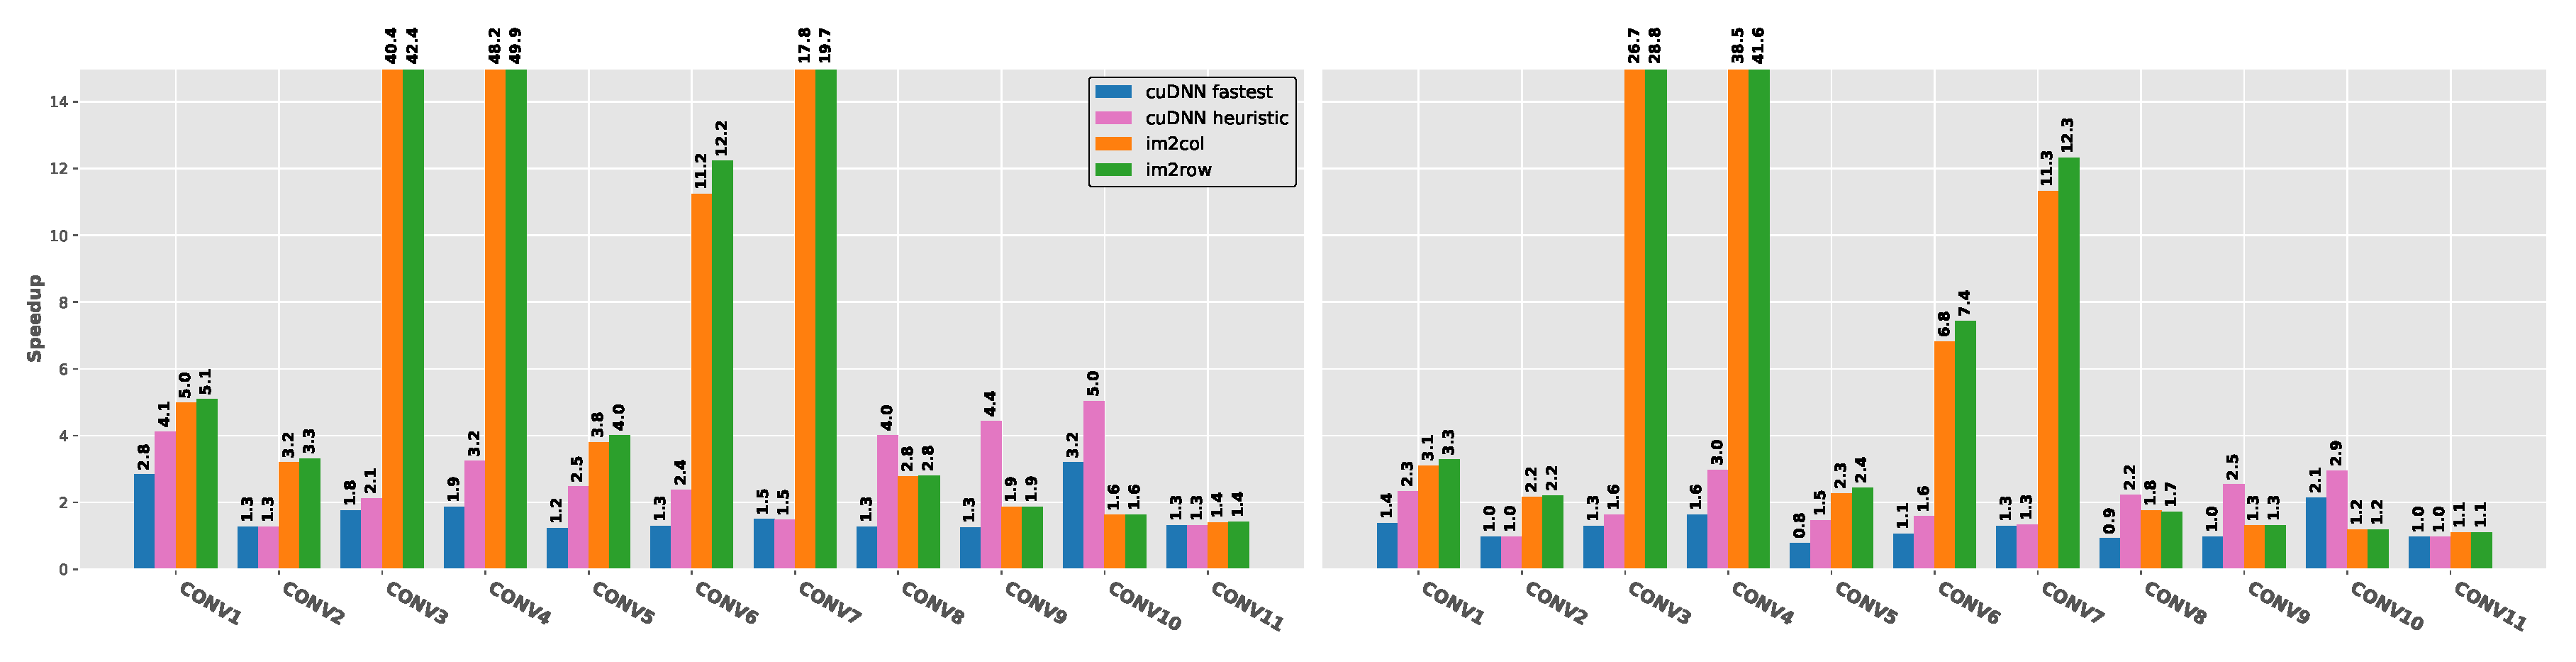
\includegraphics[width=18cm,height=5cm]{./figure/3d_norm_c1.eps}
		 %\caption{Normalized runtime of five implementations for 3D convolution. Left and right parts of the figure is for 3D convolutions with one and three input channels.}
		 %\label{fig:3druntime}
		
	\begin{subfigure}{18cm}
		\centering
		 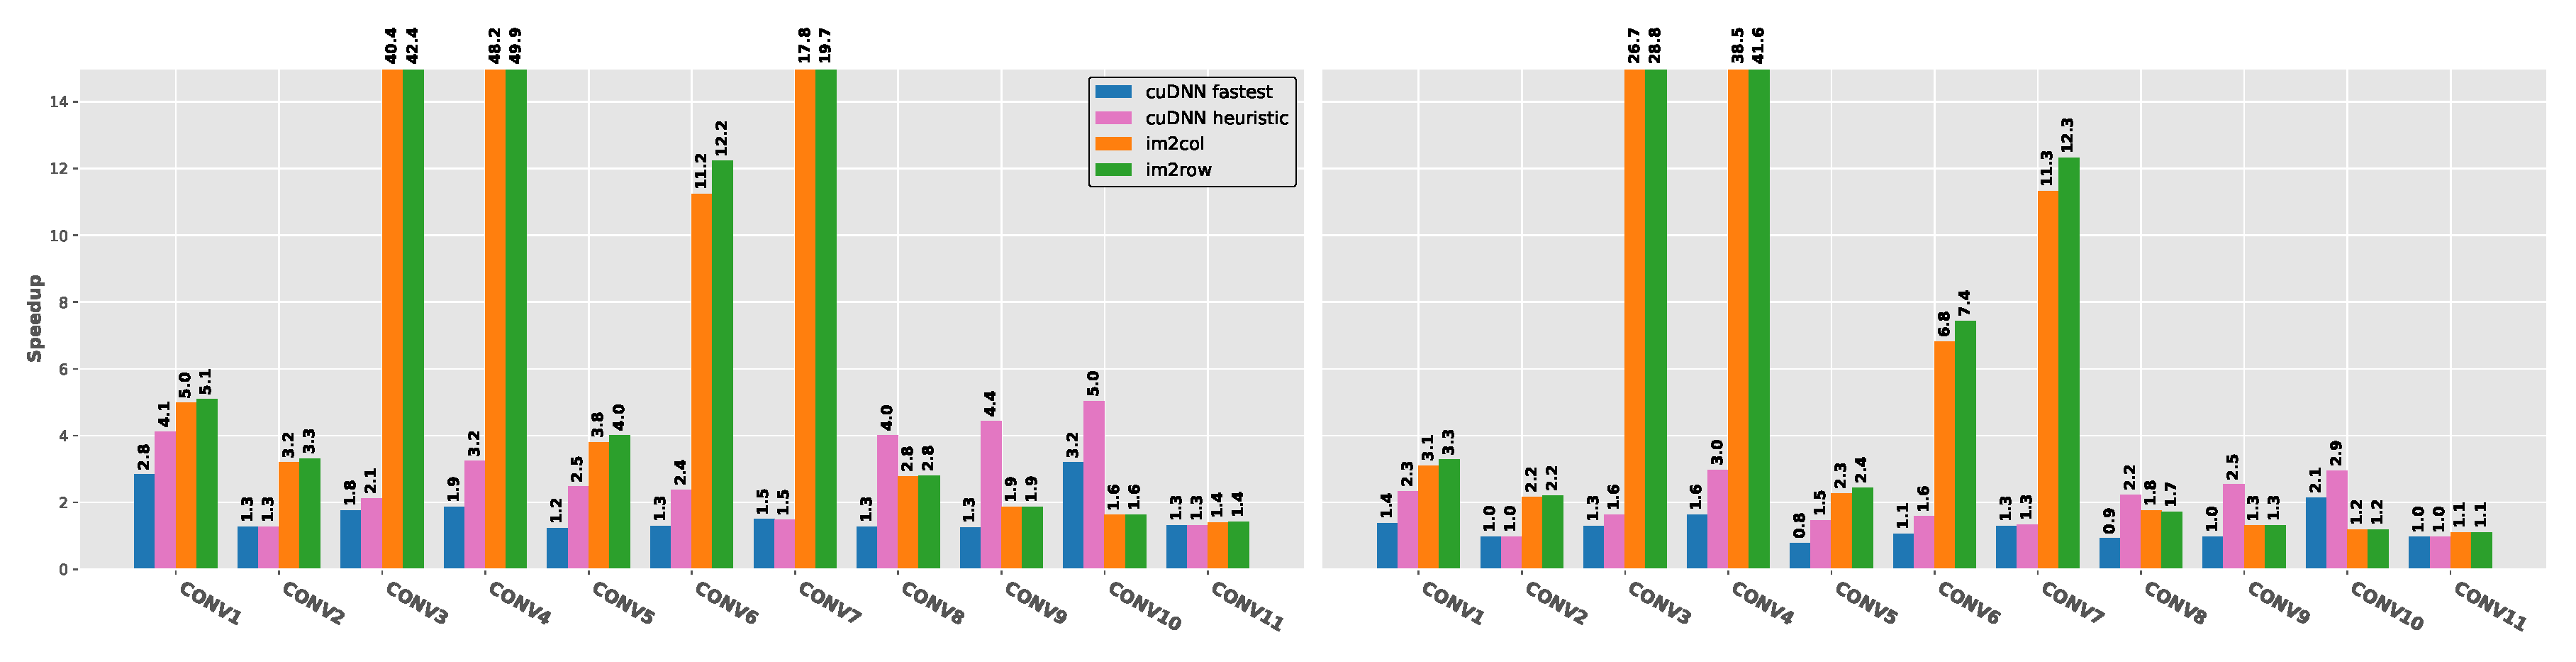
\includegraphics[width=18cm,height=5.7cm]{./figure/3d_norm_c1.eps}
		 \caption{Speedups on Tesla K40m, left is for one channel and right is for three channels.}
		 \label{fig:3druntimeK40}
	\end{subfigure}
	
	\begin{subfigure}{18cm}
		\centering
		 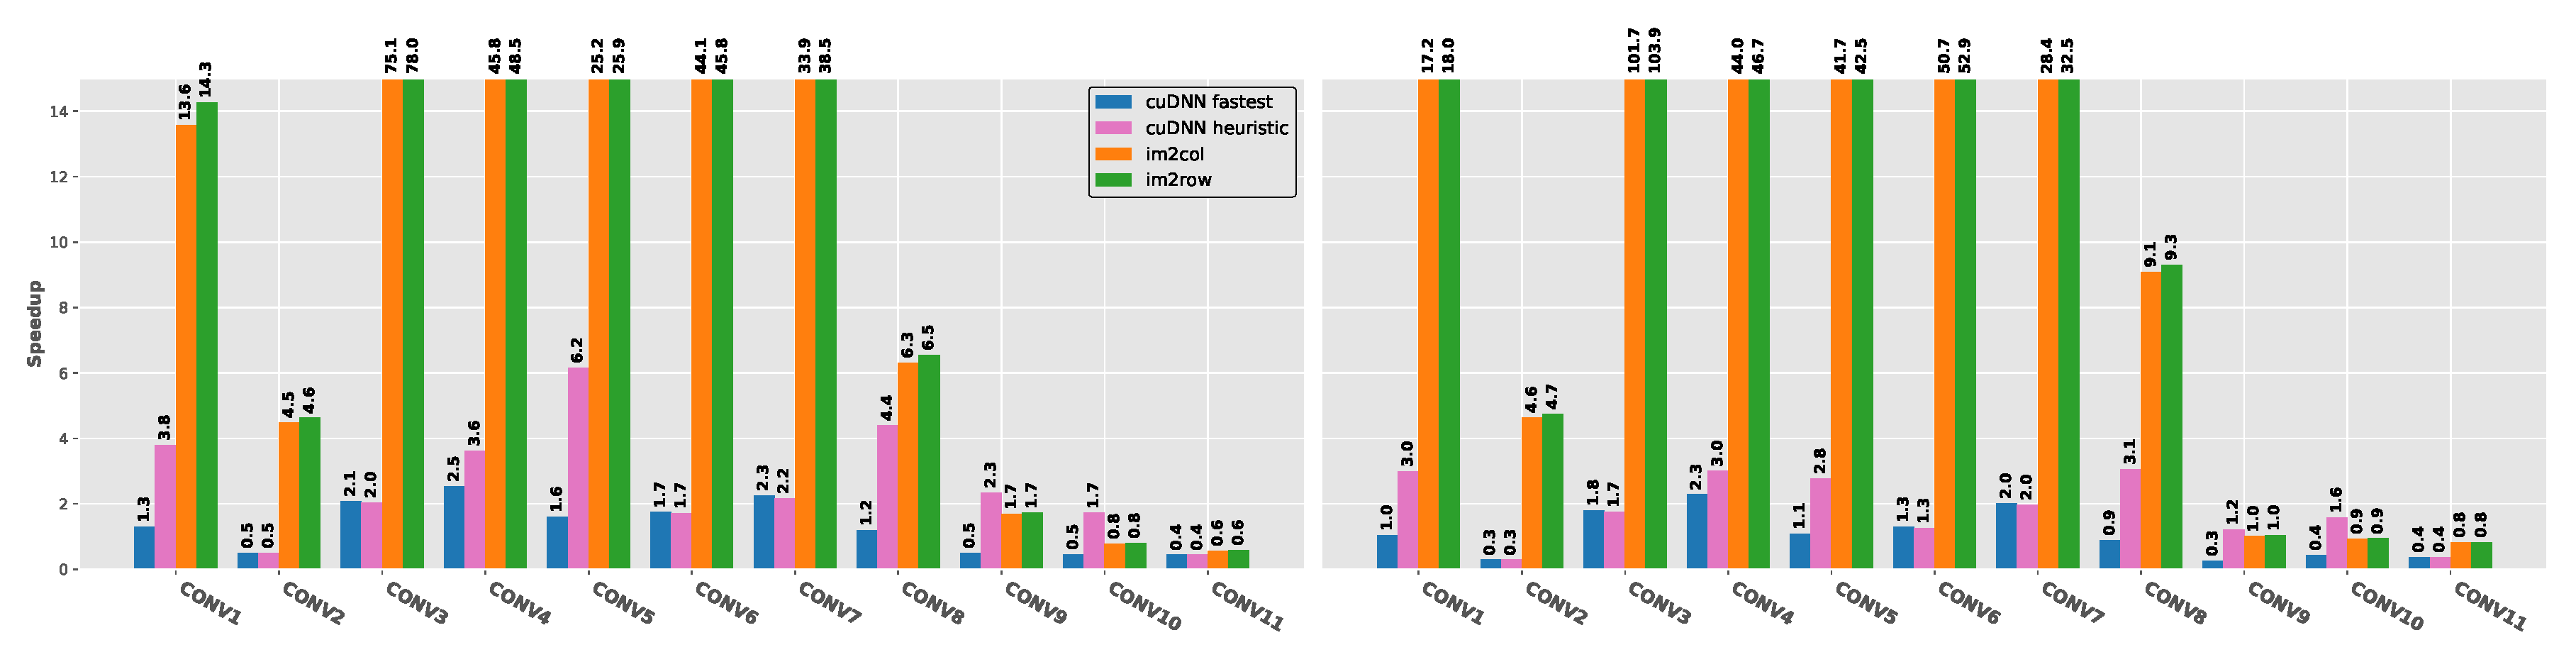
\includegraphics[width=18cm,height=5.7cm]{./figure/3d_norm_c1_rtx2080.eps}
		 \caption{Speedups on RTX 2080 Ti, left is for one channel and right is for three channels.}
		 \label{fig:3druntime2080}
	\end{subfigure}
	
	\caption{Speedups of our implementation over the other four implementations for 3D convolution with one and three input channels.}
	\label{fig:3druntime}
\end{figure*}
%\begin{figure*}
%	\begin{subfigure}{\columnwidth}
%		\centering
%		 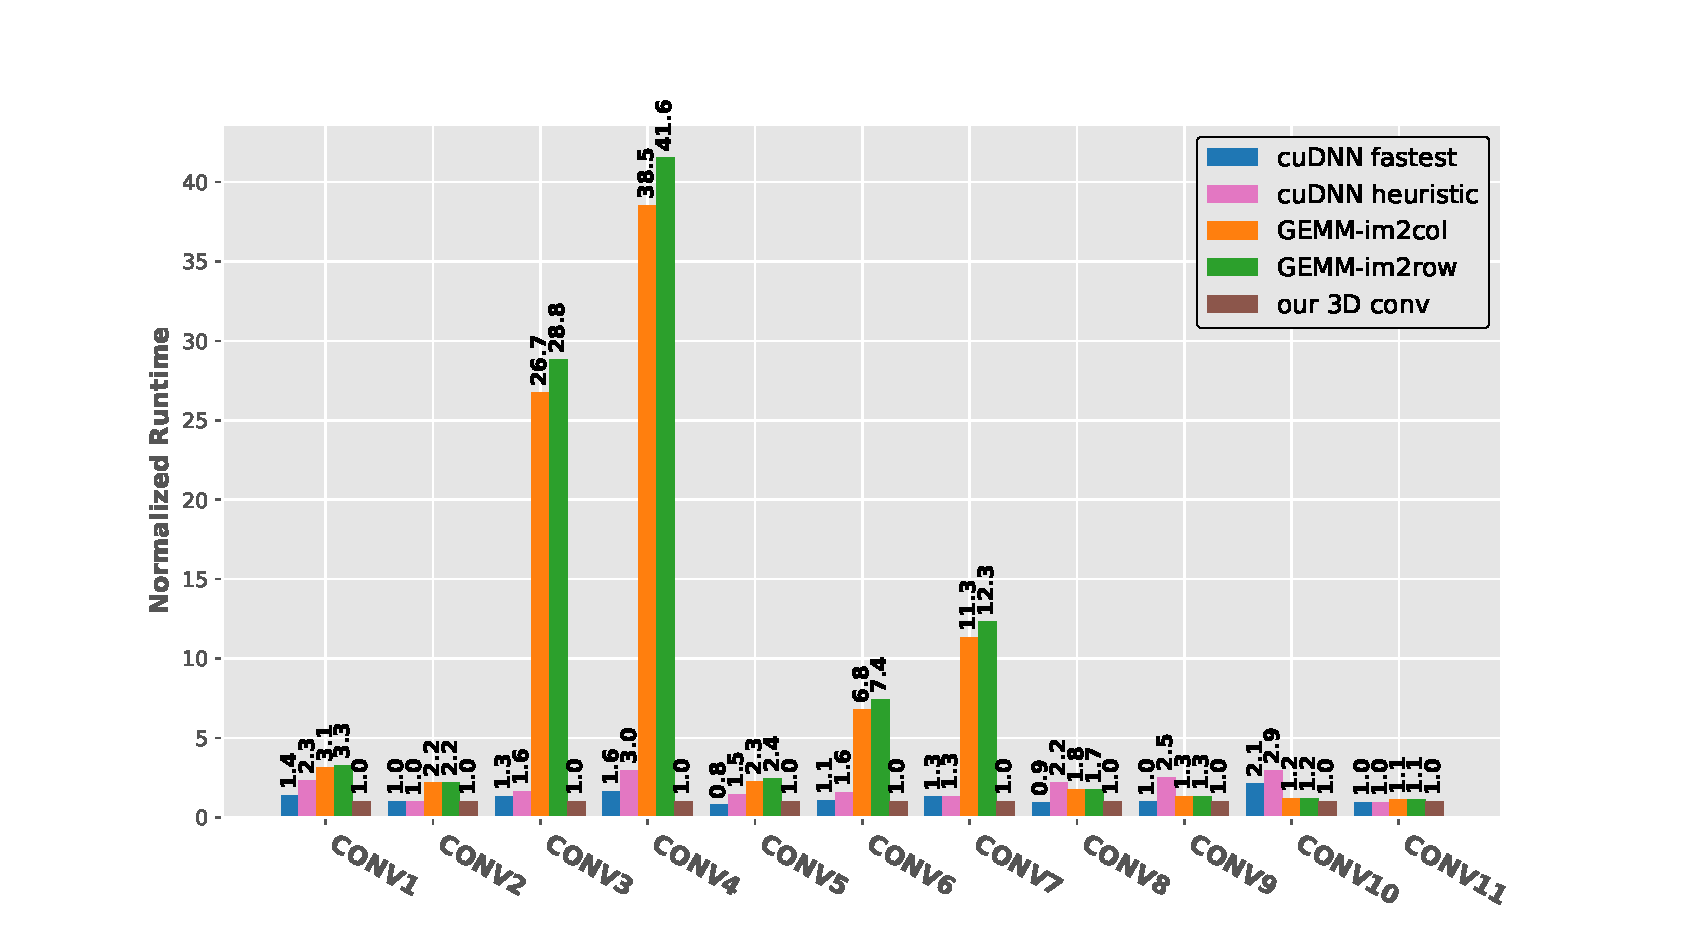
\includegraphics[width=\columnwidth,height=5cm]{./figure/3d_norm_c3.eps}
%		 \caption{Normalized runtime for convolutions with one input channel.}
%		 \label{fig:3druntimec1}
%	\end{subfigure}
%	\begin{subfigure}{\columnwidth}
%		\centering
%		 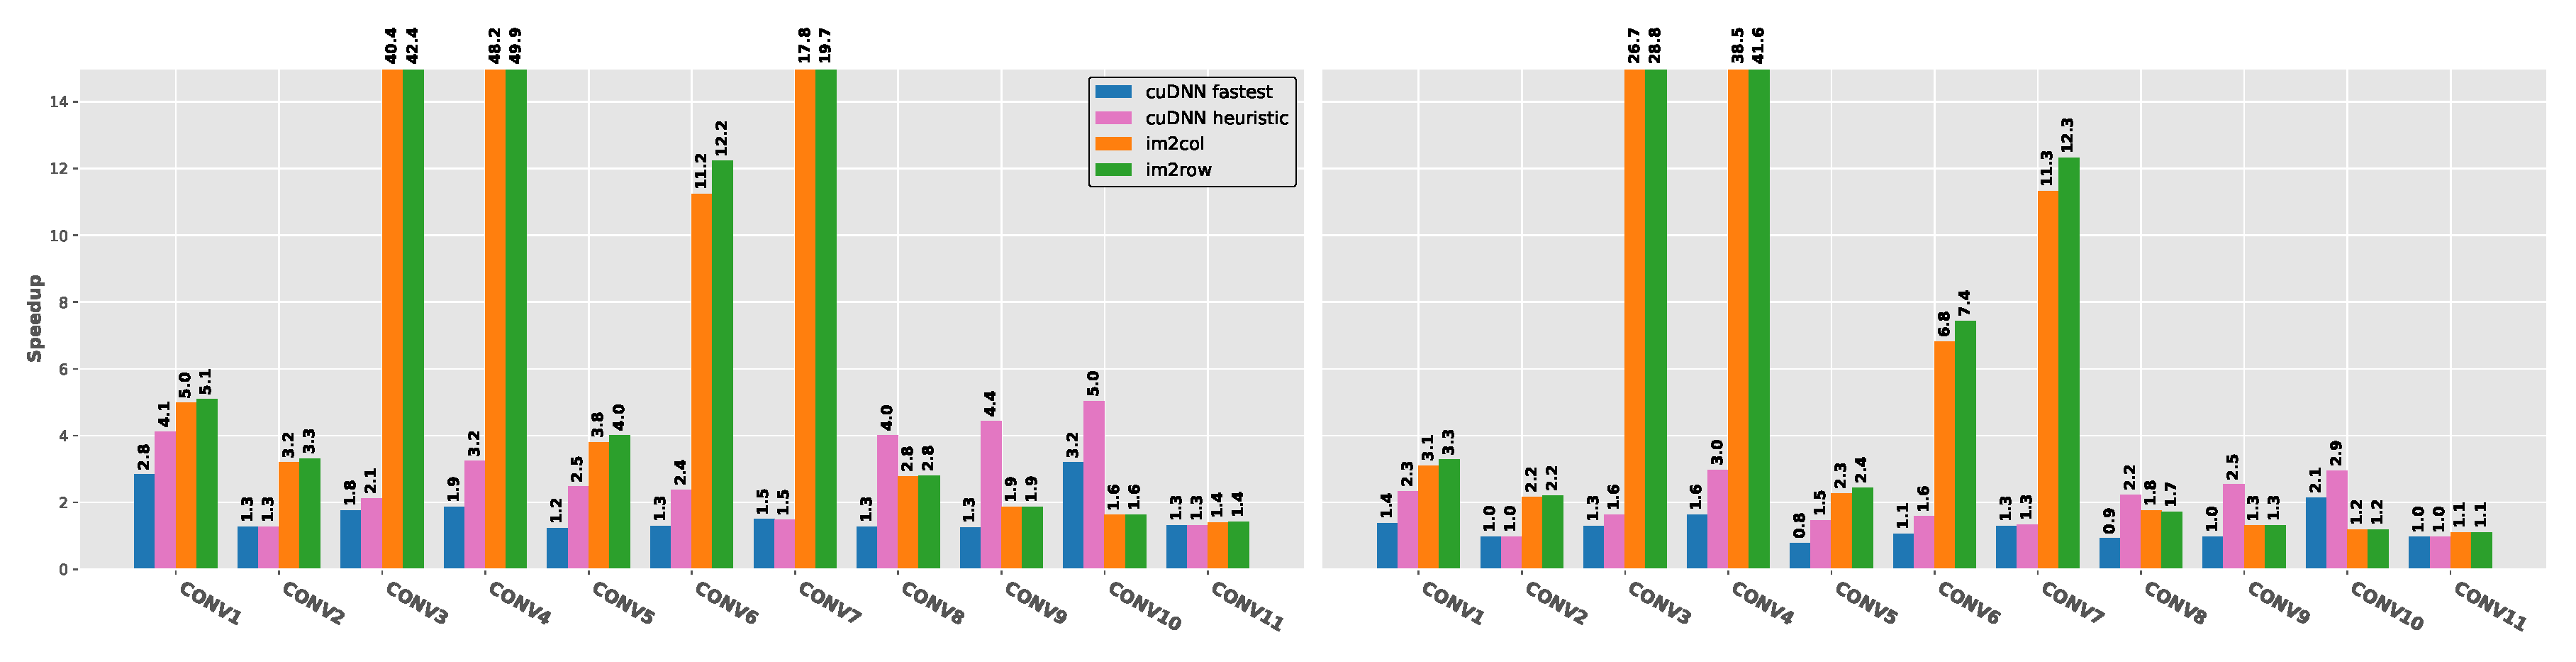
\includegraphics[width=\columnwidth,height=5cm]{./figure/3d_norm_c1.eps}
%		 \caption{Normalized runtime for convolutions with three input channels.}
%		 \label{fig:3druntimec3}
%	\end{subfigure}
%	
%	\caption{Runtime comparison among five implementations of 3D convolutions. Each runtime is normalized to our implementation.}
%   \label{fig:3druntime}
%\end{figure*}

\begin{table*}[]
\caption{The number of memory transactions for 3D convolution. Data is collected on Tesla K40m.}
\label{tab:3dtrans}
\begin{tabular}{c|ccccc|ccccc}
\hline
\multicolumn{1}{l|}{} & \multicolumn{5}{c|}{$I_C=F_C=1$}                                                                                                                                                                                                                                                                  & \multicolumn{5}{c}{$I_C=F_C=3$}                                                                                                                                                                                                                                                                  \\ \hline
    & \begin{tabular}[c]{@{}c@{}}cuDNN\\ fastest\end{tabular} & \begin{tabular}[c]{@{}c@{}}cuDNN\\ heuristic\end{tabular} & im2col & im2row & \begin{tabular}[c]{@{}c@{}}our 3D\\ conv\end{tabular} & \begin{tabular}[c]{@{}c@{}}cuDNN\\ fastest\end{tabular} & \begin{tabular}[c]{@{}c@{}}cuDNN\\ heuristic\end{tabular} & im2col & im2row & \begin{tabular}[c]{@{}c@{}}our 3D\\ conv\end{tabular} \\ \hline
CONV1& 1.7E+06& 1.2E+07& 2.3E+06& 2.3E+06& \textbf{8.5E+05}& 3.9E+06& 1.3E+07& 5.5E+06& 5.5E+06& \textbf{2.4E+06}\\
CONV2& 6.9E+06& 6.9E+06& 4.8E+06& 4.8E+06& \textbf{9.7E+05}& 1.6E+07& 1.6E+07& 1.2E+07& 1.2E+07& \textbf{2.9E+06}\\
CONV3& 3.5E+05& 1.9E+05& 1.9E+05& 2.5E+05& \textbf{8.4E+04}& 9.5E+05& 5.2E+05& 5.2E+05& 6.8E+05& \textbf{2.5E+05}\\
CONV4& 2.7E+05& 2.4E+05& 3.0E+05& 3.6E+05& \textbf{2.4E+04}& 7.4E+05& 6.4E+05& 8.0E+05& 9.8E+05& \textbf{7.3E+04}\\
CONV5& 8.7E+06& 4.5E+06& 5.1E+06& 6.5E+06& \textbf{1.4E+06}& 1.2E+07& 1.2E+07& 1.4E+07& 1.8E+07& \textbf{4.1E+06}\\
CONV6& 2.2E+06& 1.2E+06& 1.3E+06& 1.7E+06& \textbf{3.4E+05}& 5.9E+06& 3.2E+06& 3.6E+06& 4.6E+06& \textbf{1.0E+06}\\
CONV7& 1.6E+06& 1.6E+06& 1.3E+06& 1.6E+06& \textbf{1.3E+05}& 1.7E+06& 4.3E+06& 3.6E+06& 4.5E+06& \textbf{3.9E+05}\\
CONV8& 1.3E+07& 2.4E+07& 4.7E+06& 4.8E+06& \textbf{3.4E+06}& 3.0E+07& 2.9E+07& 1.1E+07& 1.2E+07& \textbf{9.8E+06}\\
CONV9& 2.7E+07& 5.5E+07& 9.9E+06& 1.0E+07& \textbf{3.9E+06}& 6.5E+07& 5.7E+07& 2.4E+07& 2.4E+07& \textbf{1.2E+07}\\
CONV10& 3.1E+07& 1.1E+08& 2.0E+07& 2.0E+07& \textbf{1.6E+07}& 7.1E+07& 1.2E+08& 5.0E+07& 5.1E+07& \textbf{4.3E+07}\\
CONV11& 1.2E+08& 1.2E+08& 7.5E+07& 7.5E+07& \textbf{2.6E+07}& 2.8E+08& 2.7E+08& 2.0E+08& 2.0E+08& \textbf{7.1E+07}\\ \hline
\end{tabular}
\end{table*}

We also apply Algorithm \ref{algo:basic}, \ref{algo:basic2} and \ref{algo:rowreuse} on a 3D convolution with one and three input channels. The focus of this study is to optimize the memory transactions, not the implementation of convolution. Thus, our convolutions do not optimize on
input channels. Algorithm \ref{algo:overalldesign} implies that the proposed implementation is in a linear scale with the number of input channels and therefore suitable for convolutions with one and three input channels, which are normally the first layers of a CNN.

In this section, we present the performance comparison of the 3D convolutions among four implementations, that is, cuDNN, im2col, im2row and our implementation. We
evaluate the performance of the 3D convolution from three aspects, speedup, number of memory transactions and memory consumption.
For cuDNN, we obtain two types of runtime. First, we run all algorithms provided in cuDNN and obtain the fastest runtime, which is denoted
as \emph{cuDNN fastest}. Second, we run cuDNN without specifying the algorithm, in which case cuDNN uses a heuristic method to find the most suitable algorithm for a convolution configuration. The runtime generated by the heuristic method is denoted as \emph{cuDNN
heuristic}. The heuristic runtime is obtained because popular machine learning frameworks, such as PyTorch, TensorFlow and Caffe,
use cuDNN with  the heuristic method in their implementations. PyThorch also uses the fastest algorithm of cuDNN in some cases.

\begin{figure*}
	
	\begin{subfigure}{\columnwidth}
		\centering
		 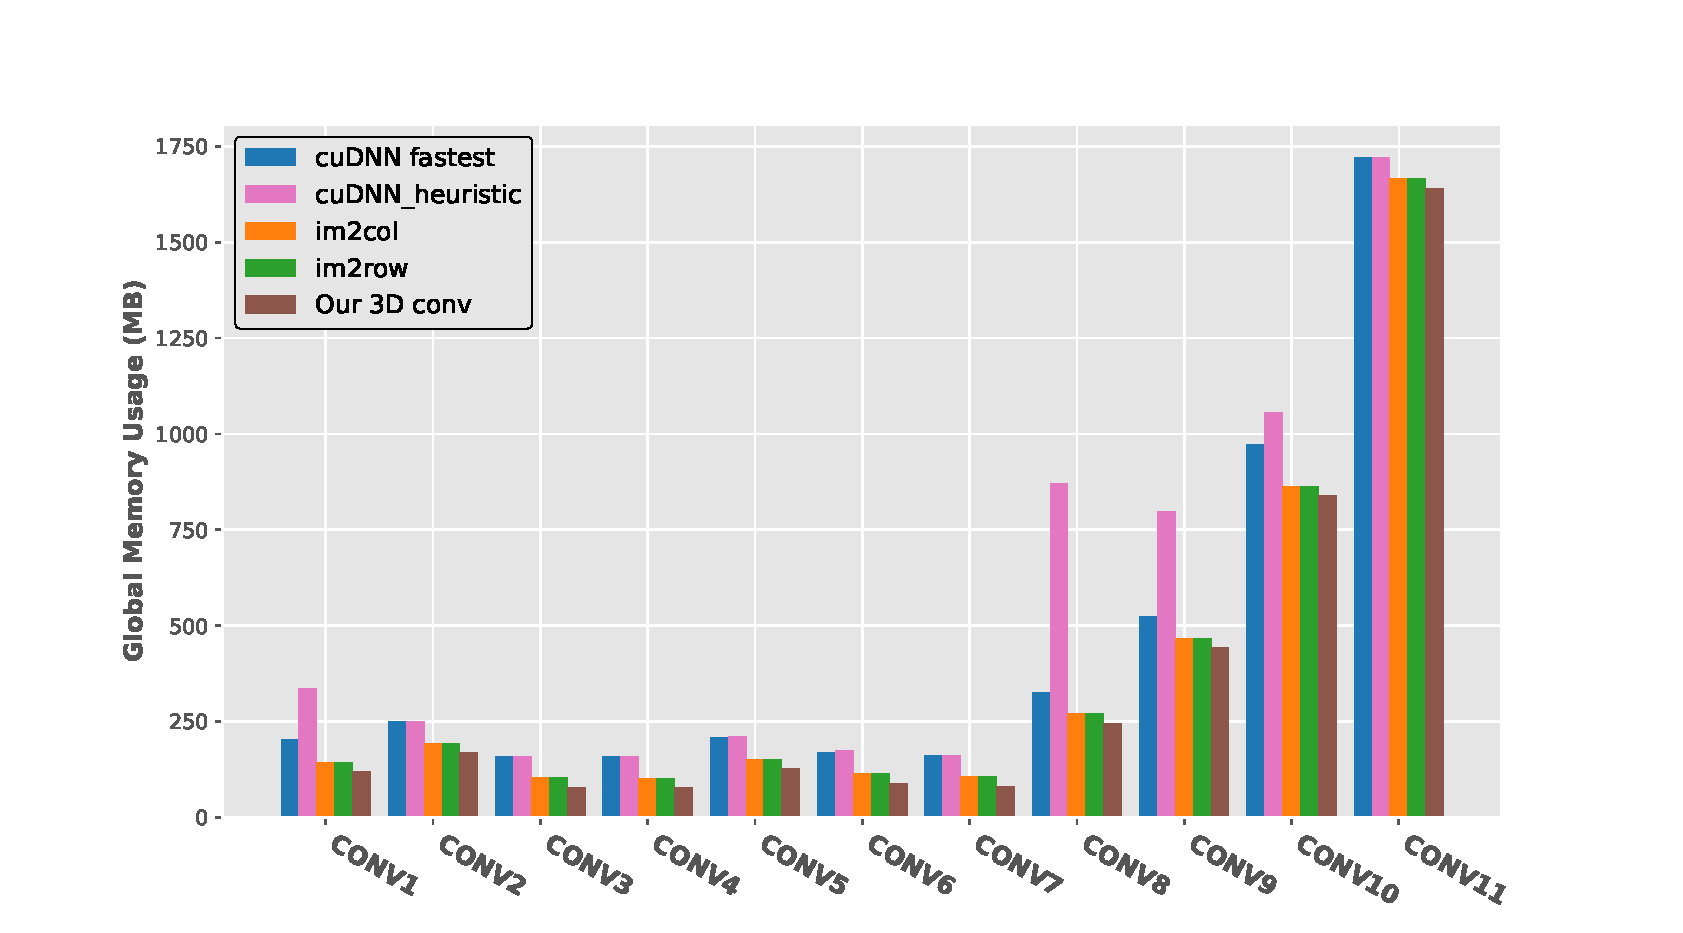
\includegraphics[width=\columnwidth,height=6cm]{./figure/mem3d_1.eps}
		 %\caption{Global memory usage for five implementations on Tesla K40m.}
		 \label{fig:3dmemk40m}
	\end{subfigure}
	\begin{subfigure}{\columnwidth}
		\centering
		 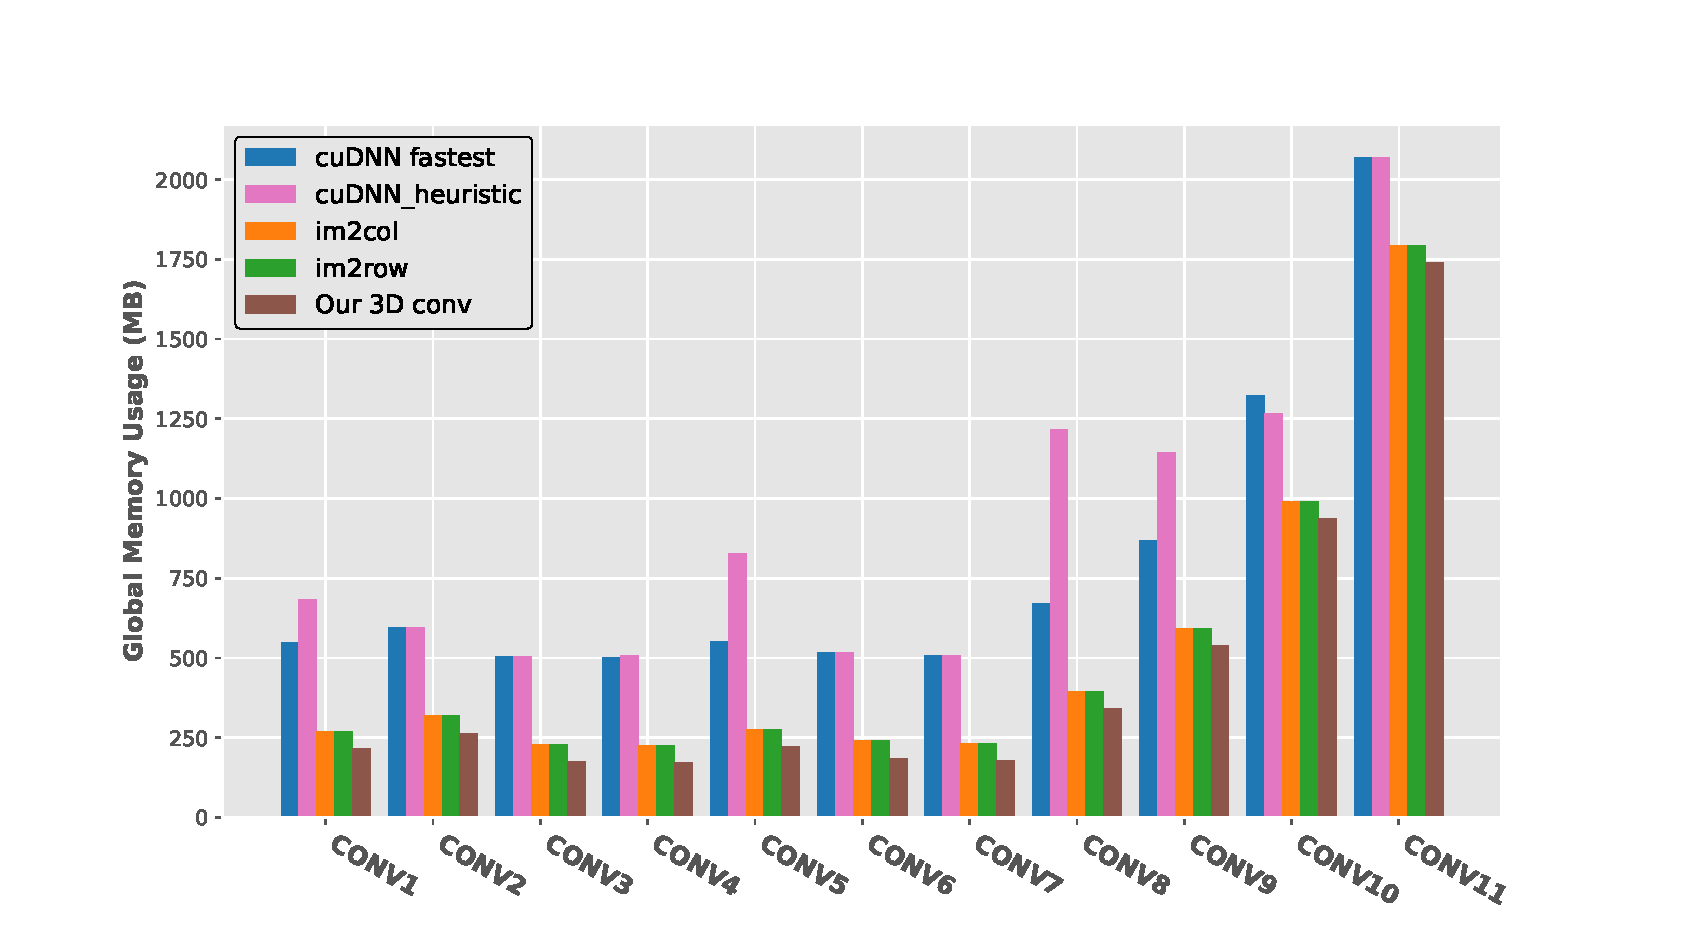
\includegraphics[width=\columnwidth,height=6cm]{./figure/mem3d_1_rtx2080.eps}
		 %\caption{Global memory usage for five implementations on RTX 2080 Ti.}
		 \label{fig:3dmemrtx2080}
	\end{subfigure}
	\caption{Global memory usage for five implementations. Left figure demonstrates the result on Tesla K40m and right figure demonstrates the result on RTX 2080 Ti.}
	\label{fig:3dmem}
\end{figure*}

We collect the configurations of the convolutional layers using $3 \times 3$ and $5 \times 5$ filers from four popular CNN models,
namely, AlexNet \cite{Krizhevsky2012ImageNet}, VGG \cite{SimonyanZ14a}, ResNet \cite{HeZRS16} and GoogleLeNet \cite{SzegedyLJSRAEVR15}.
Then, we set the number of input channels to one and three ($I_C=F_C \in \{1, 3\}$) and the batch size to 128 ($I_N=O_N=128$). Other batch
sizes demonstrate a similar performance because all tested implementations have a linear scale as the batch size. The exact configuration is presented in Table \ref{tab:3dconvconfigs}.

We test all the 3D convolution implementations on two platforms, and the speedups of our implementation over the other four implementations are shown
in Figure \ref{fig:3druntime}. We can see that im2col and im2row perform poorly in most cases, especially on RTX 2080 Ti. Our
implementation achieves average speedups of 17.9$\times$ and 18.8$\times$ relative to im2col and im2row on the two platforms, respectively. Figure \ref{fig:3druntimeK40} displays the speedups on Tesla K40m. Although cuDNN is well optimized for 3D convolutions on GPU, our implementation exceeds the speed of the former by an average of 1.5$\times$ and 2.3$\times$ with respect to cuDNN fastest and cuDNN heuristic, respectively. The speedups on RTX 2080 Ti are shown in Figure \ref{fig:3druntime2080}. Compared with cuDNN fastest, the proposed approach achieves an average speedup of 1.2$\times$, with the maximum speedup reaching 2.5$\times$. The speedup over cuDNN heuristic is higher at 2.2$\times$, and the maximum speedup can reach up to 6.2$\times$.

In contrast to 2D convolutions, the performance gains of 3D convolutions are obtained from two aspects: reduction of the memory transactions of the input data and filters. After loading a filter into the shared memory, we use it to slide over as many images as possible to eliminate the need to load the same filter for each input. Table \ref{tab:3dtrans} lists the number of memory transactions in the four implementations on Tesla K40m. We use the same method used in the 2D convolution to collect the number of memory transactions. Our approach achieves
the minimum transaction counts in all tested cases and can reduce the number of memory transactions by a factor of 6.1 and 4.4
with respect to \emph{cuDNN fastest} with one and three input channels, respectively. Compared with the transaction counts in 2D convolution (Table \ref{tab:2dmemtrans}), that in the 3D convolution has a lower ratio than the other implementations. This phenomenon occurs because in 3D convolutions, each filter needs to slide over all inputs. Hence, we need to load the same filter multiple times. Although we have optimized the use of filters, we still need to load the filters multiple times because the capacity of the shared memory cannot fit the entire
filters. Consequently, the number of memory transactions increases.

For 3D convolutions, memory usage is important for the scarce memory storage in GPU. We use \emph{nvidia-smi} command to record the peak GPU device memory usage when the application is running. In this study, we only report the global memory usage for the
convolutions with one input channel because output data consumes the most memory storage compared with the input and filter data. In addition, changing the number of input channels alone does not change the size of the output data. Therefore, memory usage exhibits only a slight change when we change the number of input channels.

Figure \ref{fig:3dmem} illustrates the memory usage of the four implementations on two platforms. Our implementation is derived from direct convolution, which does not require extra memory, and therefore consumes the minimum memory storage. GEMM-based implementations (im2col and im2row) first transform the filters into a large matrix before transforming one input into a matrix when performing a matrix multiplication. Therefore, such implementations only need extra memory to store the transformed filters and the transformed input. The most memory consuming
implementation is cuDNN. Considering that cuDNN is a closed source, we can only guess that this approach improves the performance at the expense of memory usage. The
memory consumption of our implementation is reduced by 335 MB on average, with the maximum reduction reaching 384 MB with respect to cuDNN fastest. The commonly used
cuDNN heuristic consumes even more memory than cuDNN fastest. Compared with the cuDNN heuristic, our implementation reduces  memory consumption by 442 MB on average, with the maximum reduction reaching up to 876 MB.

In summary, our optimization algorithms can reduce the number of memory transactions and improve the performance of 3D convolutions on the two platforms. In contrast to cuDNN, which consumes a large amount of substantial memory to accelerate the convolution operation, especially for the cuDNN heuristic, the proposed implementation does not need any extra memory.
%From Table \ref{tab:3dspeedup} we can see that as the channel number increases, the speedup of cuDNN, im2col and im2row decrease obviously. We analyze the algorithms of im2col and im2row. Both transform the channels into a large matrix and the use the highly optimized gemm library to do the real work. When we increase the number of channels, the size of the transformed matrix also increases. But the gemm library can distribute the work among gpu cores very well, which brings little overhead on each gpu core. Though without the source code of cuDNN, we use $nvprof$ to analyze cuDNN and find that cuDNN also utilizes gemm library to do the real work. Therefore the reason also holds for cuDNN. In our implementation, we loop over each channel to calculate the final result. As the channel number increases, out implementation shows a linear scale as channel number. Therefore, as the channel number increases, the speed up of our implementation over cuDNN, im2col and im2row decreases. ArrayFire uses a similar method as our implementation, the speedup over ArrayFire is not decreased. Further optimization on channel number will be explored in the future. In this work, we mainly focus on the effectiveness of our two reuse algorithms not the implementation of the convolution.

%Second, compare through 3*3 and 5*5, we can find that for cudnn im2col im2row npp 's sppedup keep same across different filter size, but ArrayFire decreasees, the reason is that when compailing for filter 5, we have to reduce the number of each thread. or it will generate
